% % APÊNDICES--------------------------------------------------------------------

\begin{apendicesenv}
\partapendices

% % Primeiro apêndice------------------------------------------------------------
\chapter{Protótipo do Aplicativo Mobile} % Edite para alterar o título deste apêndice
\label{chap:apendiceA}

\begin{figure}[h]
    \centering
    \caption{Tela de Login, sincronização e menu principal}
    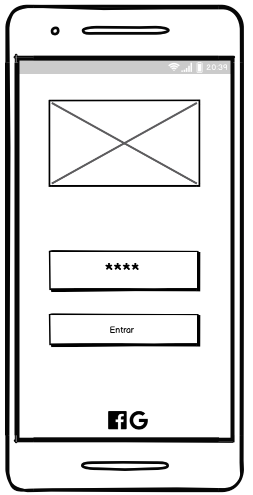
\includegraphics[width=0.3\textwidth]{./dados/figuras/p1.png}
    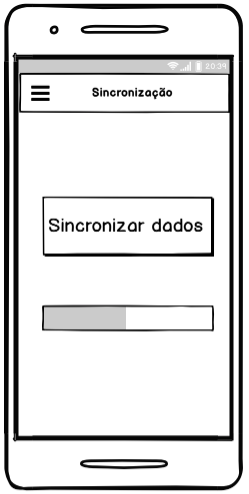
\includegraphics[width=0.3\textwidth]{./dados/figuras/p2.png}
    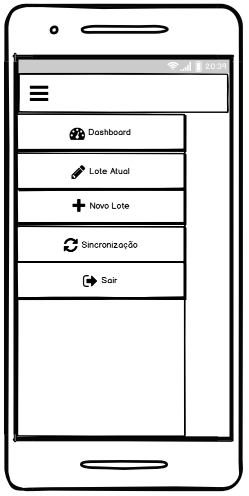
\includegraphics[width=0.3\textwidth]{./dados/figuras/p3.png}
    \fonte{Autor}
    \label{fig:p1}
\end{figure}

\begin{figure}[h]
    \centering
    \caption{Tela do lote atual e registro de mortalidade}
    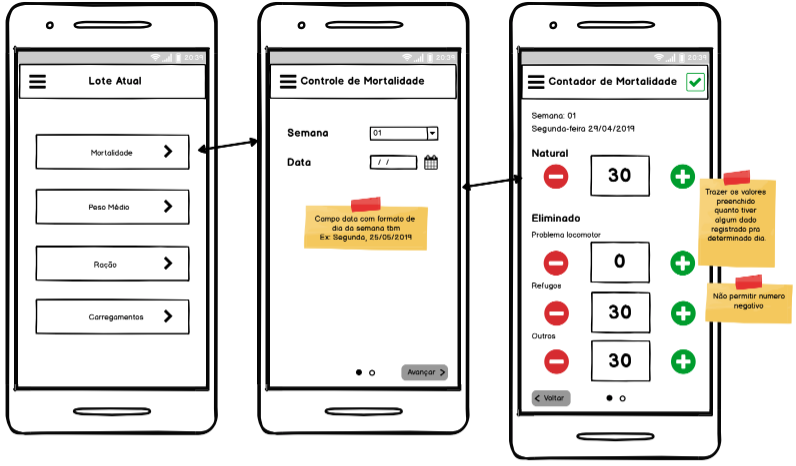
\includegraphics[width=1.0\textwidth]{./dados/figuras/p4.png}
    \fonte{Autor}
    \label{fig:p4}
\end{figure}

\begin{figure}[h]
    \centering
    \caption{Tela de registro de pesagem}
    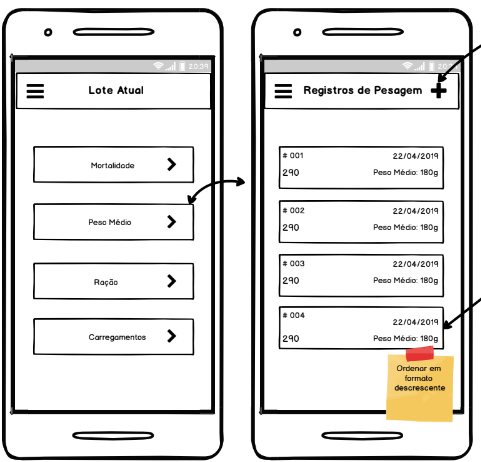
\includegraphics[width=0.8\textwidth]{./dados/figuras/p5.png}
    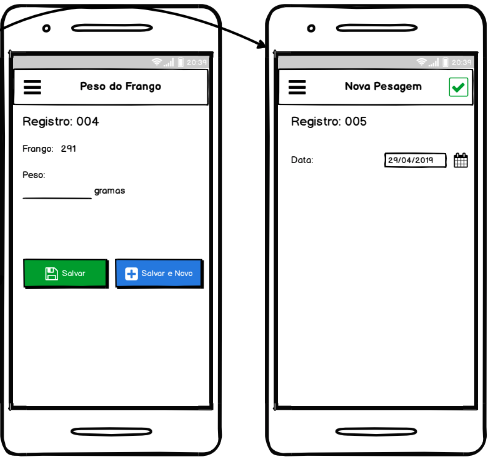
\includegraphics[width=0.8\textwidth]{./dados/figuras/p5_1.png}
    \fonte{Autor}
    \label{fig:p5}
\end{figure}

\begin{figure}[htb!]
    \centering
    \caption{Tela do dashboard}
    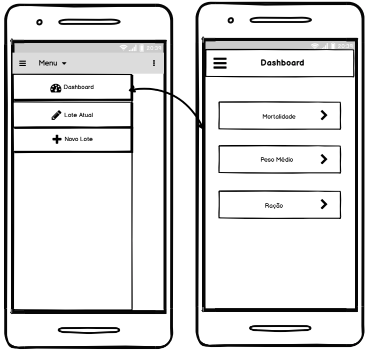
\includegraphics[width=0.8\textwidth]{./dados/figuras/p6.png}
    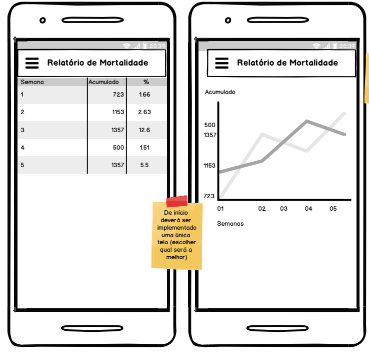
\includegraphics[width=0.8\textwidth]{./dados/figuras/p7.png}
    \fonte{Autor}
    \label{fig:p6}
\end{figure}

% Lembre-se que a diferença entre apêndice e anexo diz respeito à autoria do texto e/ou material ali colocado.

% Caso o material ou texto suplementar ou complementar seja de sua autoria, então ele deverá ser colocado como um apêndice. Porém, caso a autoria seja de terceiros, então o material ou texto deverá ser colocado como anexo.

% Caso seja conveniente, podem ser criados outros apêndices para o seu trabalho acadêmico. Basta recortar e colar este trecho neste mesmo documento. Lembre-se de alterar o "label"{} do apêndice.

% Não é aconselhável colocar tudo que é complementar em um único apêndice. Organize os apêndices de modo que, em cada um deles, haja um único tipo de conteúdo. Isso facilita a leitura e compreensão para o leitor do trabalho.

% % Novo apêndice----------------------------------------------------------------
% \chapter{APÊNDICE}
% \label{chap:apendiceB}
% Teste3
% conteúdo do novo apêndice
\end{apendicesenv}
